\chapter{Упругое когерентное рассеяние нейтрино и методы его регистрации} \label{chapt1}
В течение ХХ века была разработана одна из величайших физических теорий — Стандартная Модель. Данная теория объединила в себе все известные на момент своего создания элементарные частицы, а также предсказала новые, которые впоследствии были открыты.
\par Современная экспериментальная физика элементарных частиц отличается большим разнообразием как предметов так и методов исследования. Цели этих экспериментов варьируются от проверки предсказаний Стандартной Модели и уточнения ее параметров до поиска подтверждений расширения существующих теорий и “новой физики”.  Среди экспериментов присутствуют классические ускорительные, главным из которых, безусловно, является Большой Адронный Коллайдер; космофизические наземные и орбитальные эксперименты; эксперименты по исследованию темной материи~\cite{Cebrian:2022brv}, нейтринные эксперименты. Регистрация и исследование свойств нейтрино является одной из самых сложных задач в экспериментальной физике. Вместе с тем, это одно из самых перспективных направлений.
\section{Упругое когерентное рассеяние нейтрино на атомных ядрах} \label{sect1_1}
\subsection{Теория}
\label{subsect1_1_1}
В рамках электрослабой теории был предсказан процесс упругого когерентного рассеяния нейтрино. Процесс был почти одновременно предсказан зарубежными и отечественными учеными в работах~\cite{Freedman, Kopeliovich:1974mv} в 1974 году. 

В данном случае нейтрино рассеивается одновременно на всех нуклонах ядра. Такое возможно в том случае если длина волны нейтрино заметно превышает физические размеры ядра, то есть ... >> 1~\cite{Freedman:1977xn}. При одновременном и когерентном (с совпадающими фазами) рассеивании на нескольких рассеивателях амплитуда процесса возрастает в A раз, где A -- количество рассеивателей, то есть нуклонов. Соответственно, полное сечение процесса оказывается усиленным в A$^2$ раз. Однако, данные наивные рассуждения справедливы только в случае .... Если принять во внимание различные направления спина у нуклонов, то формула сечения примет вид:

Таким образом, учитывая что (приближения всякие) реальной увеличение сечения оказывается равным $N^2$ раз, где $N$ --- число нейтронов в ядре.

Отличительной чертой процесса является то, что нейтрино вступает во взаимодействие со всеми нуклонами ядра когерентным образом, что приводит к увеличению сечения взаимодействия примерно в $N^2$ раз, где $N$ --- число нейтронов в ядре. Данный процесс представляет собой обмен $Z$-бозоном между нейтрино и всеми нуклонами ядра одновременно.
\begin{figure}[h]
	\center{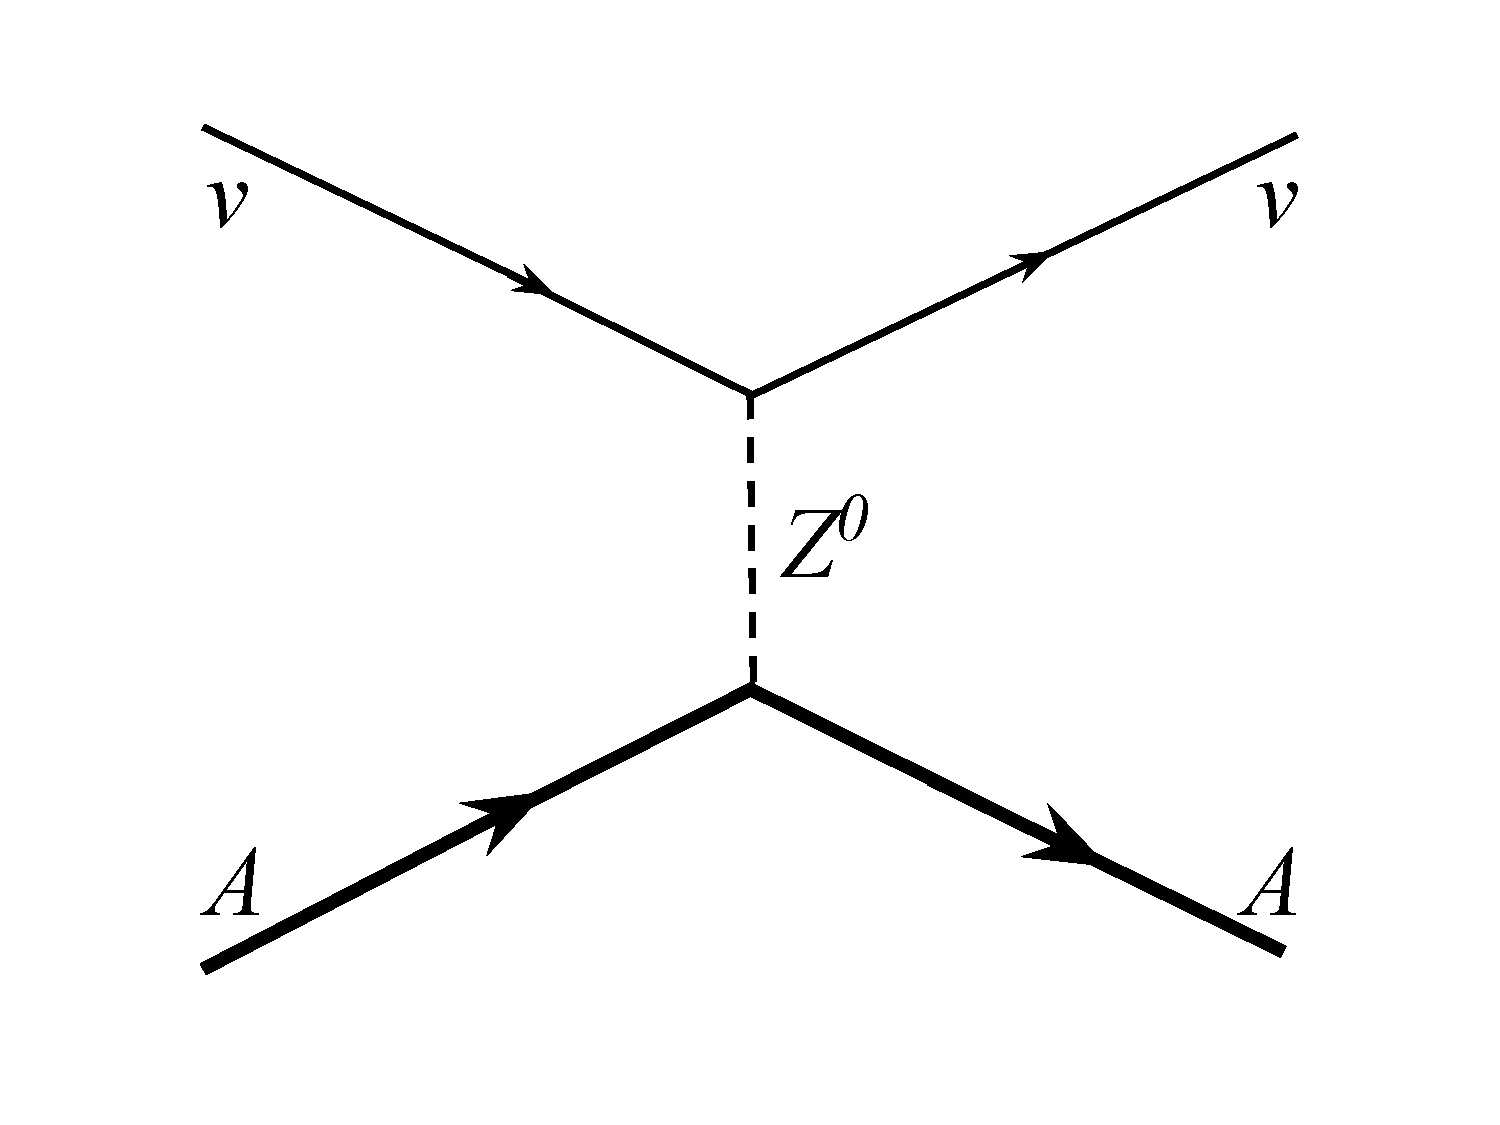
\includegraphics[width=0.6\linewidth]{images/cevns.pdf}}
	\caption{Схема когерентного рассеяния нейтрино на ядре}
	\label{ris:cevns}
\end{figure}
\par Дифференциальное сечение процесса представляется формулой \cite{cevns1, Lindner2017}:
	
\begin{equation}
\frac{d\sigma}{dE_r} = \frac{G_f^2}{4\pi} Q_w^2M\left(1-\frac{ME_r}{2E_\nu}\right)F^2(Q^2),
\end{equation}\\
	
	где $G_f$ --- константа Ферми;
	$Q_w=N-(1-4\sin^{2}\theta_w)Z$ --- слабый заряд для ядра с числом нуклонов $N$ и зарядом ядра $Z$;
	$F(Q^2)$ --- форм-фактор;
	$\theta_w$ --- угол смешивания слабого взаимодействия (угол Вайнберга).
	Используя значение угла можно показать, что сечение взаимодействия
	 $\sim N^2$:\\
	 
	$\sin^2(Q_w)\approx 0.22$ $\to Q_w\sim N \to \sigma \sim N^2$\\
	
	Полное сечение процесса приближённо равно:\\
	
	$\sigma \approx 0.4\cdot10^{-44}  N^2$(E$_\nu^2)$см$^{2}$/МэВ. \\
	\par
	Процесс УКРН имеет место при энергии нейтрино менее 50 МэВ, когда длина волны де Бройля для нейтрино не превосходит размеры ядра, и взаимодействие идет когерентно.
	Отметим, максимальная энергия ядра отдачи равна
\begin{equation}
    T_{max} = \frac{2E_{\nu}^{2}}{M+2E_{\nu}},
    \label{Tmax}
\end{equation}
то есть для большинства элементов энергия ядра отдачи очень мала --- порядка единиц-десятков кэВ на ядро. Таким образом возникают серьезные экспериментальные трудности при регистрации подобных процессов.
\subsection{Эксперименты по исследованию УКРН}
\label{subsect1_1_2}
Долгое время, несмотря на наличие теоретического предсказания, эксперименты по исследованию упругого когерентного рассеяния нейтрино не проводились. Это связано с экстремально низкой, как следует из формулы \ref{Tmax} (единицы-десятки кэВ) энергией ядра отдачи, что предъявляет серьезные требования к экспериментам, уровням шумов электроники и внешних фонов. В последние годы прогресс в области низкофоновых экспериментов сильно шагнул вперед во многом благодаря возросшему интересу к темной материи. 
\par Впервые процесс УКРН был зарегистрирован коллаборацией COHERENT в 2017 году на детекторе CsI[Na]~\cite{COHERENT:2017ipa}. Эксперимент коллаборации COHERENT был поставлен на ускорителе SNS в Окриджской Национальной Лаборатории в США. %Молекулы Cs и I имеют очень близкие атомные номера (78 и 74), что приводит к тому, что эффективный атомный номер позволяет сделать достоверные выводы о зависимости сечения от характер данного процесса от атомного номера по полученным данным. 
Через несколько лет успех коллаборации был повторен и УКРН было зарегистрировано на ядрах аргона \cite{PhysRevLett.126.012002}, что позволяет сделать достоверные выводы о зависимости сечения от характер данного процесса от атомного номера по полученным данным. На данный момент в мире существует более 10 экспериментов по исследованию УКРН. Среди них есть эксперименты как на ускорителях \cite{COHERENT:2018gft}, так и на реакторах \cite{Belov_2015, Aguilar-Arevalo_2016, ricochet, Buck_2020, Singh:2016glu, Strauss_2020, Chaudhuri:2022pqk}. 

\section{Двухфазный метод регистрации частиц} 
\label{sect1_2} 
\subsection{История создания и основной принцип работы}
\label{sect1_2_1}
Детекторы на сжиженных благородных газах разной сложности использовались в экспериментальной физике для регистрации частиц много лет \cite{Chepel_2013}. Благородные газы, такие как аргон и ксенон отличаются рядом преимуществ, которые позволяют масштабировать детекторы до большого (вплоть до нескольких тонн рабочего вещества) объема, регистрировать события малой (единицы-десятки кэВ) энергии. Кроме того, они легко поддаются очистке за счет своей инертности.  В 1970 году Б.А. Долгошеиным был предложен~\cite{Dolgoshein} метод, основанный на использовании двух фаз рабочего вещества. Схема работы метода изображена на рисунке \ref{img:twophase}.

\begin{figure}[h]
	\center{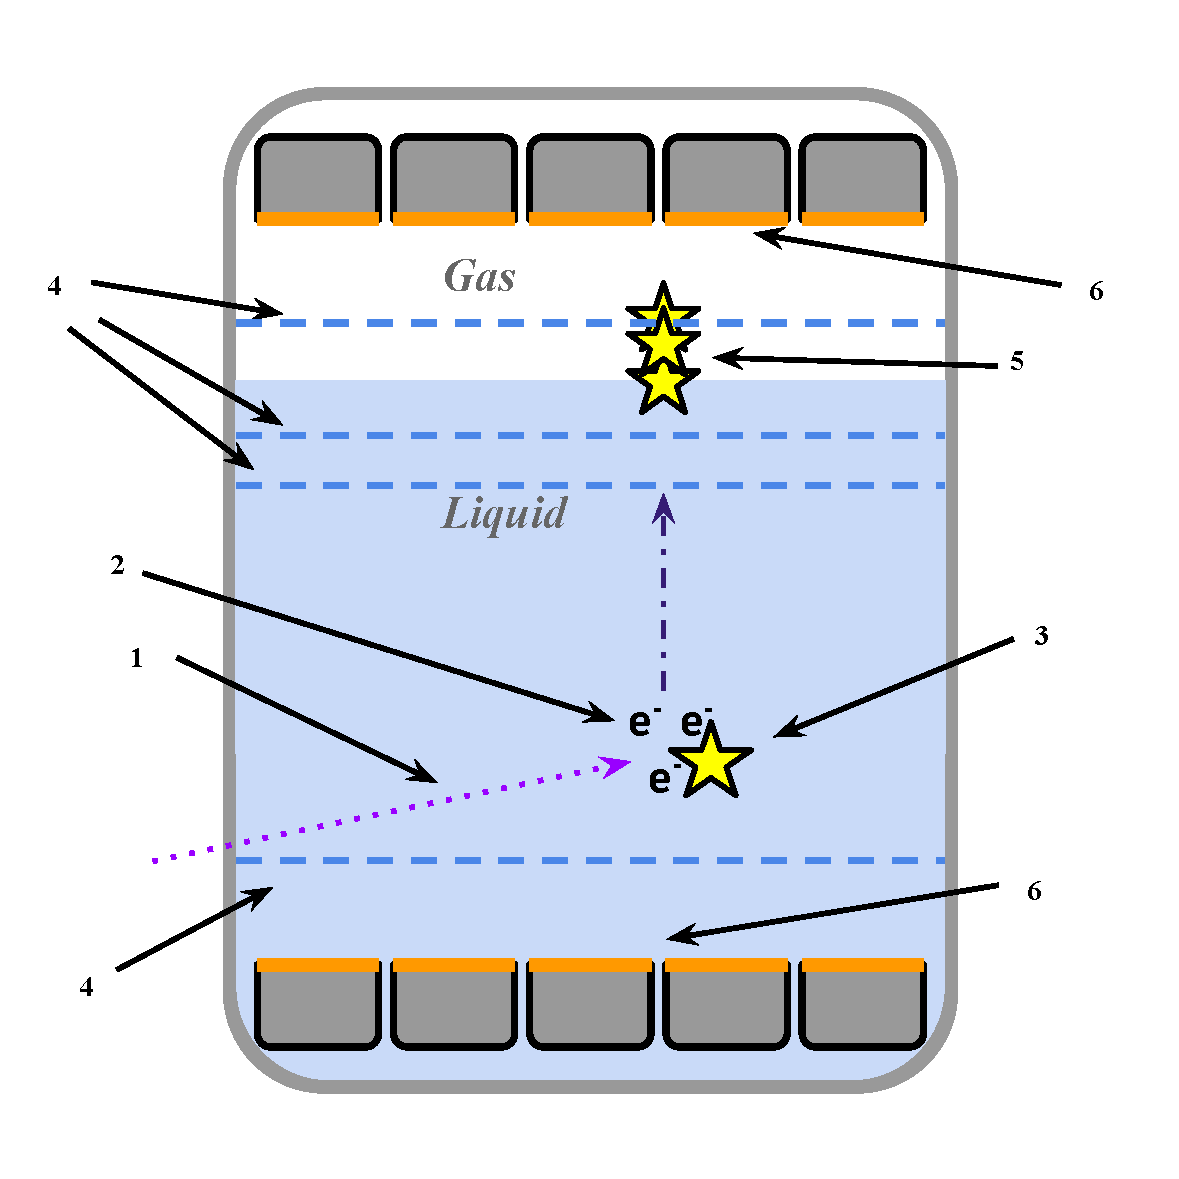
\includegraphics[width=0.7\linewidth]{images/twophasedetector.pdf}}
	\caption[Схема работы двухфазного детектора.] {1 -- трек ионизирующей частицы; 2 -- электроны ионизации, возникшие в результате взаимодействия; 3 -- вспышка сцинтилляции (S1), возникшая в результате взаимодействия; 4 -- электроды-сетки, создающие напряжение; 5 -- электролюминесценция (S2) в электролюминесцентном зазоре; 6 -- матрицы из фотоумножителей}
	\label{img:twophase}
\end{figure}

При взаимодействии элементарной частицы с ксеноном испускаются фотоны сцинтилляции (S1) и электроны ионизации.  Электроны ионизации под действием приложенного электрического поля дрейфуют к границе раздела фаз. После выхода в газовую газе электроны возбуждают атомы ксенона с излучением вторичной сцинтилляции (S2), также называемой электролюминесценцией. Следует подчеркнуть, что размножение электронов отсутствует, следовательно количество фотонов пропорционально количеству электронов. Регистрация сцинтилляции и электролюминесценции происходит за счет фотоумножителей, расположенных сверху и снизу от рабочего объема. Временной промежуток между S1 и S2 вкупе с информацией о скорости дрейфа электронов позволяют рассчитать глубину произошедшего события, а распределение света по матрицам фотоумножителей — координаты в горизонтальной плоскости и полную энергию события. Трехмерная реконструкция событий позволяет создавать так называемые детекторы  "без стенок"\, выделяя внутри детектора отдельный рабочий объем (FV - fiducial volume), содержащий малое количество событий из внешнего фона, что особенно важно если речь идет о поиске редких событий с низкой энергией.

\subsection{Двухфазные детекторы в современной экспериментальной физике}
\label{sect1_2_2}
Двухфазные детекторы нашли широкое применение в низкофоновой физике. В основном это эксперименты по исследованию темной материи~\cite{BOLOZDYNYA2015405}. Первым двухфазным детектором "без стенок" был XENON10, содержащий 5 кг жидкого ксенона в FV. Этот детектор послежил прототипом проектов XENON100~\cite{Xenon10} и XENON1T~\cite{Xenon100}, содержащих 100 и 1100 кг жидкого ксенона в FV, соответственно. Также ксенон в качестве рабочего вещества используется в детекторах экспериментов LUX, Zeplin, LZ~\cite{LZ} и Panda-X~\cite{Xiao:2017vys}. Жидкий аргон используется в экспериментах DarkSide~\cite{DarkSide:2014llq}, DUNE~\cite{Chardonnet_2020}.
\par Отличительной чертой всех экспериментов по исследованию темной материи явлется расположение глубоко под землей. Толща породы обеспечивала естественное экранирование от космических лучей. Детектор РЭД-100 раполагался на поверхности Земли, что потребовало модификации двухфазного метода регистрации с учетом повышенного фона от космических мюонов. 